\documentclass[10pt,letterpaper]{article}

\usepackage{ccn}
\usepackage{pslatex}
\usepackage{apacite}

\title{Analyzing disentanglement of visual objects in semi-supervised neural networks}
 
\author{{\large \bf Andrew David Zaharia$^\star$ (andrew.z@columbia.edu)} \\
  Mortimer B. Zuckerman Mind Brain Behavior Institute\\
  Columbia University, New York, NY 10027, USA
  \AND {\large \bf Benjamin Peters$^\star$ (benjamin.peters@columbia.edu)} \\
  Mortimer B. Zuckerman Mind Brain Behavior Institute\\
  Columbia University, New York, NY 10027, USA
  \AND {\large \bf John Cunningham (jpc2181@columbia.edu)} \\
  Department of Statistics and Grossman Center\\
  Columbia University, New York, NY 10027, USA
  \AND {\large \bf Nikolaus Kriegeskorte (n.kriegeskorte@columbia.edu)} \\
  Mortimer B. Zuckerman Mind Brain Behavior Institute\\ Departments of Psychology, Neuroscience, and Electrical Engineering\\
  Columbia University, New York, NY 10027, USA
  \AND $^\star$ These authors contributed equally to this work}

%% AZ additions
\usepackage{graphicx,xcolor}
\graphicspath{{./figures/}}

% \hyphenation{auto-encoder}
\hyphenation{auto-encoders}
% \hyphenation{dis-entangle}
\newcommand{\bvae}{$\beta$-VAE~}

\begin{document}

\maketitle

\section{Abstract}
{
\bf
A fundamental goal of visual systems is to condense visual stimuli into compact representations of relevant information they contain. Ideally, these representations would consist of the independent ``generative factors'' that fully determine, on a semantic level, the visual input. Such a ``disentangled'' representation could consist of the identity of a background scene, and the identity, position, pose, and size of an object. Recent research in deep neural networks (DNNs) has focused on achieving disentangled representations, through unsupervised learning, of single objects or faces in isolation. We trained and analyzed a popular DNN model of disentanglement, the $\beta$-variational autoencoder ($\beta$-VAE) on a new dataset, containing a ``foreground'' white circle and ``background'' isotropic Gaussian. We show that the neural network autoencoder architecture we use can achieve prefect disentanglement with supervised learning, but only achieves partial disentanglement when using the unsupervised \bvae loss function. On our dataset, higher $\beta$ results in higher reconstruction loss and greater entanglement. We propose that further inductive bias is needed to achieve better disentanglement, such as a representation which factorizes static properties and their dynamics.
}
\begin{quote}
\small
\textbf{Keywords:} 
disentanglement; unsupervised learning; deep neural network; autoencoder; object vision
\end{quote}


\section{Introduction}

Neural \textit{selectivity} and \textit{invariance} both increase at higher levels in the visual hierarchy \cite{Rust2010}. Here, ``selectivity'' refers to how finely a neuron can discriminate different stimulus representations in a particular feature space, and ``invariance'' refers to how tolerant the neuron is to changes in other stimulus properties. The result of these computations is the \textit{disentangling} of visual representations to ones which compactly and independently encode the true generative factors of the world \cite{DiCarlo2007}. In object recognition for example, such factors could be the object's identity, size, rotation, lighting, and color. This same concept of disentanglement has been proposed as a desirable final representation in deep neural networks (DNNs) and an explanation of the types of features found in intermediate DNN layers \cite{Bengio2009}.

Recent work on disentanglement in DNNs has focused on the unsupervised learning setting. The $\beta$-variational autoencoder (\bvae) claimed to learn more disentangled representations by treating the reconstruction error term in the VAE loss function as a regularizer \cite{Higgins2017,Kingma2014}. By deemphasizing reconstruction error, \bvae and related methods \cite{Alemi2017,Mathieu2018} place a tighter bottleneck on the information that can be represented, which can sometimes lead to less entangled representations. These approaches, however, are quite general and do not necessarily lead to truly disentangled representations.


\section{Experiments}

\begin{figure}%[t!]
  % \begin{center}
     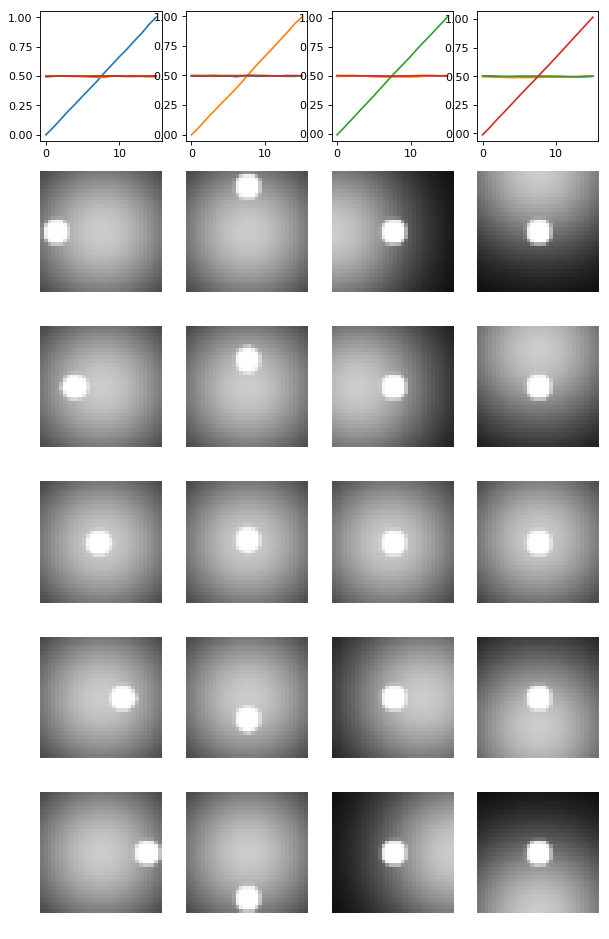
\includegraphics[width=3.375in]{entangle_analysis_supervised_anddata.png}
     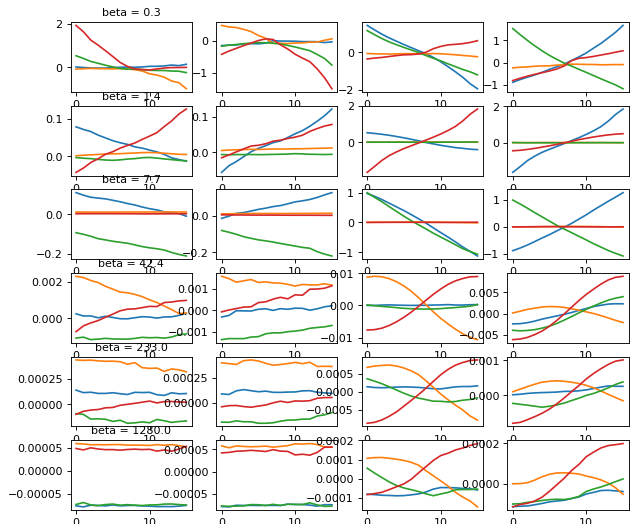
\includegraphics[width=3.375in]{entangle_analysis_betaVAE.png}
  % \end{center}
  \caption{\textbf{Circle+Gaussian dataset and varying levels of entangled representations.}}{(a) The circle+Gaussian dataset, with one generating factor changing in each column (from left to right: circle horizontal and vertical locations, Gaussian horizontal and vertical locations). (b) A perfectly disentangled representation. As one generative factor linearly increases, one unique latent variable also linearly increases while the rest are constant. (c) In entangled representations, as one generative factor changes, multiple latent factors change.}
  \label{fig:dataset}
\end{figure}

We first assessed the level of disentanglement existing models can achieve in extremely simple settings where perfect disentanglement should be achievable by creating a new, simple dataset (see figure~\ref{fig:dataset}a). We randomly varied the positions of each object while keeping size and intensity fixed. Therefore, there are 4 generative factors for this dataset: the horizontal and vertical position of each object. An ideal encoder for these images that is perfectly disentangled is one with four latent variables, where each one uniquely maps to one of the four generative factors (see figure~\ref{fig:dataset}b). An entangled representation would be one in which multiple latent variables change when varying a single generative factor, and potentially nonlinearly (see figure~\ref{fig:dataset}c).

As a basic control, we wanted to verify that a perfectly disentangled encoder could be achieved by training a simple encoder network with supervision to map its four latent variables directly to the generative factors. The encoder network has four convolutional layers, each with a stride of 2, and a rectified linear (ReLU) output nonlinearity. It is followed by a fully connected layer that maps to the four latent factors. Figure~\ref{fig:dataset}b indeed shows the results from this experiment, demonstrating that this architecture is capable of representing the underlying generative factors in a disentangled way.

Next, we trained \bvae with the same encoder network architecture and a decoder network with the size-matched fully connected and deconvolutional layers in reverse, for different $\beta$ values. The resulting representations are entangled (figure~\ref{fig:dataset}c), and become less informative for higher $\beta$ values.

% \begin{figure}[t!]
%   % \begin{center}
%      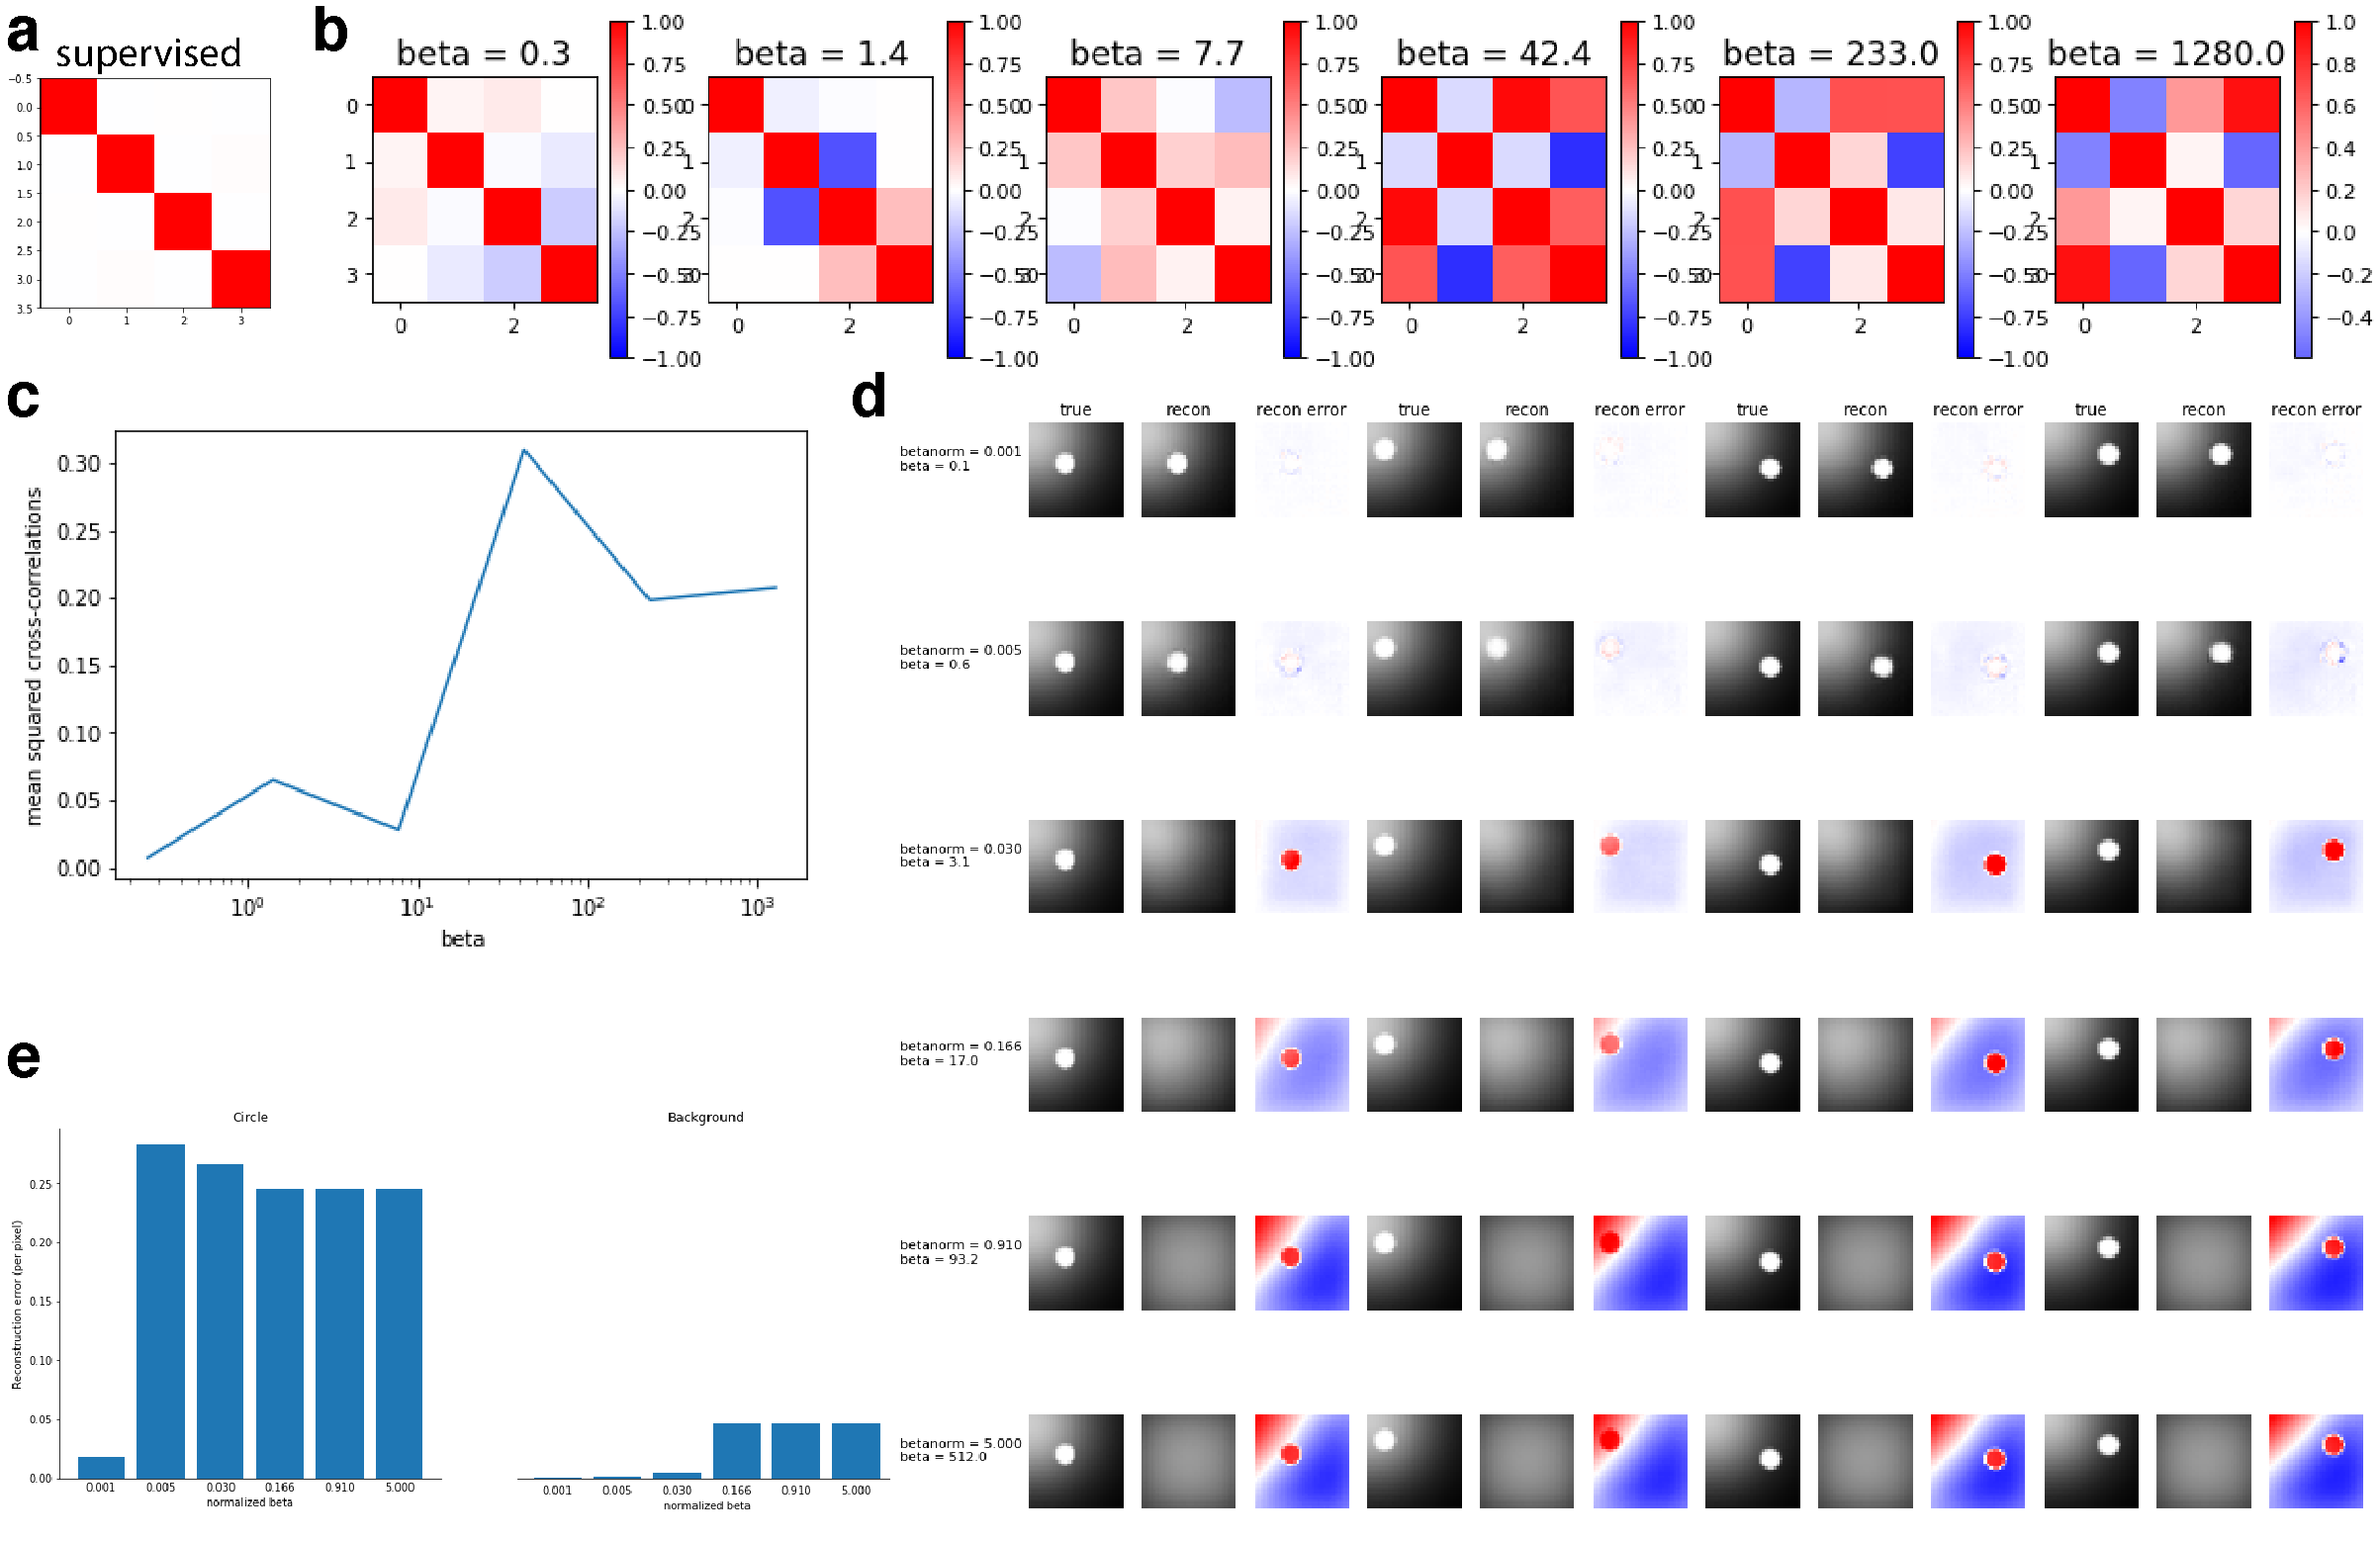
\includegraphics[width=3.375in]{analyses.pdf}
%   % \end{center}
%   \caption{\textbf{\bvae latent correlation analyses and reconstructions. [PLACEHOLDER!]}}{(a) Supervised encoder latent variable correlations in response to the experiments depicted in figure~\ref{fig:dataset}a show no covariation: they are perfectly disentangled. (b) The same plot as (a), but for \bvae with different $\beta$ values. (c) The mean of the squared off-diagonal entries in the correlation matrices shown in (b). Covariation of latent variables increases with increasing $\beta$, indicating increasing entanglement. (d) For each column containing three images, the left most is the true input image, the middle is the \bvae reconstruction, and on the right is the difference between the two. Note that the circle objects disappear from the reconstructions for all but the lowest two $\beta$ values. (e) Reconstruction error per pixel, as a function of $\beta$, computed either on pixels inside the circle (left) or outside (right).}
%   \label{fig:analyses}
% \end{figure}

% Another way to assess entanglement is to ask how correlated each latent variable is with the other latent variables (figure~\ref{fig:analyses}(a-b)). The representation learned through supervised training shows no correlations between latents. For increasing $\beta$, \bvae latents showed increasing correlations with each other (figure~\ref{fig:analyses}(b-c)). Reconstructions from the \bvae models, however, were good for the lowest two $\beta$s tested, but systematically failed for higher $\beta$ (figure~\ref{fig:analyses}d). Specifically, with increasing $\beta$, first, the white circle completely disappeared but the Gaussian was still reproduced reasonably well. Further increasing $\beta$, the Gaussian was also replaced by a similar shape that is always centered, consistent with the notion that the network has reached its ``auto-decoding'' limit, where the latents are completely ignored \cite{Alemi2017}. This was further quantified with the observation that reconstruction loss on our circles and Gaussians dataset, considered on a per-pixel basis, reaches higher levels for the circle than for the background at lower $\beta$s (figure~\ref{fig:analyses}e).
% % In order to assess the effects of adding dynamics into models of disentanglement, we created a dynamic version of the dataset that comprised linear motion of the foreground circle.  ...


\section{Conclusion}

With these simulations, we hope to lay the foundation for using DNN methods for unsupervised and semi-supervised learning to probe how disentangled representations of objects could emerge. The level of disentanglement and reconstruction quality in \bvae further declined with increasing $\beta$. This is somewhat at odds with previous predictions, in which one should trade-off with the other \cite{Higgins2017,Alemi2017}, but is likely due to our choice of a low number of latent variables.

We hypothesize that a further inductive bias is necessary to produce truly disentangled representations. Objects are not static; they exist in a continuous world. The putative generative factors that determine an object’s appearance are likely to remain stable (e.g., the object's identity) or vary smoothly and slowly over time (e.g., the object's position or rotation) \cite{Wiskott2002}. This inductive bias could support feature learning in biological systems. We propose that a representation which factorizes static properties and their dynamics will lead to better disentanglement.

\bigskip

%\section{Acknowledgments}
%Place acknowledgments (including funding information) in a section at
%the end of the paper.

\bibliographystyle{apacite}
\setlength{\bibleftmargin}{.125in}
\setlength{\bibindent}{-\bibleftmargin}
\bibliography{refs}

\end{document}
